\chapter{Machine Learning Models}
\label{ch:modeles}

\section{Linear Regression}
\label{sec:regression_lineaire}

\index{linear regression}

\begin{definition}[Linear Regression]
\textbf{Linear regression} models the relationship between a target variable $y$ and explanatory variables $\mathbf{x}$:
\[
y = \mathbf{X}\boldsymbol{\beta} + \varepsilon
\]
where $\boldsymbol{\beta}$ is the coefficient vector and $\varepsilon$ is the error term.
\end{definition}

\begin{theorem}[Ordinary Least Squares (OLS)]
\index{ordinary least squares}\index{OLS}
The OLS estimator minimizes the sum of squared residuals:
\[
\hat{\boldsymbol{\beta}} = \arg\min_{\boldsymbol{\beta}} \| \mathbf{y} - \mathbf{X}\boldsymbol{\beta} \|^2 = (\mathbf{X}^\top \mathbf{X})^{-1}\mathbf{X}^\top \mathbf{y}
\]
\end{theorem}

\begin{definition}[Coefficient of Determination $R^2$]
\index{coefficient of determination}\index{R squared@$R^2$}
The $R^2$ measures the proportion of variance explained by the model:
\[
R^2 = 1 - \frac{\sum_{i=1}^{n}(y_i - \hat{y}_i)^2}{\sum_{i=1}^{n}(y_i - \bar{y})^2} \in (-\infty, 1]
\]
An $R^2$ close to 1 indicates a good fit.
\end{definition}

\begin{codeblock}[title=\textbf{Python}]
\begin{minted}{python}
import seaborn as sns
import pandas as pd
from sklearn.linear_model import LinearRegression
from sklearn.model_selection import train_test_split
from sklearn.metrics import mean_squared_error, r2_score

# Load the tips dataset
tips = sns.load_dataset('tips')
X = tips[['total_bill', 'size']]
y = tips['tip']

X_train, X_test, y_train, y_test = train_test_split(
    X, y, test_size=0.3, random_state=42
)

# Linear regression
reg = LinearRegression()
reg.fit(X_train, y_train)
y_pred = reg.predict(X_test)

print(f"Coefficients: {reg.coef_}")
print(f"Intercept:    {reg.intercept_:.4f}")
print(f"R\u00b2 (test):    {r2_score(y_test, y_pred):.4f}")
print(f"RMSE (test):  {mean_squared_error(y_test, y_pred, squared=False):.4f}")
\end{minted}
\end{codeblock}

\begin{codeoutput}
\begin{minted}{text}
Coefficients: [0.0932 0.1803]
Intercept:    0.6689
R² (test):    0.4616
RMSE (test):  1.0459
\end{minted}
\end{codeoutput}

\section{Logistic Regression}
\label{sec:regression_logistique}

\index{logistic regression}\index{sigmoid}

\begin{definition}[Logistic Regression]
\textbf{Logistic regression} is a \textbf{binary classification}\index{binary classification} model. It models the probability of belonging to class 1 via the sigmoid function:
\[
P(y=1 \mid \mathbf{x}) = \sigma(\mathbf{x}^\top \boldsymbol{\beta}) = \frac{1}{1 + e^{-\mathbf{x}^\top \boldsymbol{\beta}}}
\]
\end{definition}

\begin{center}
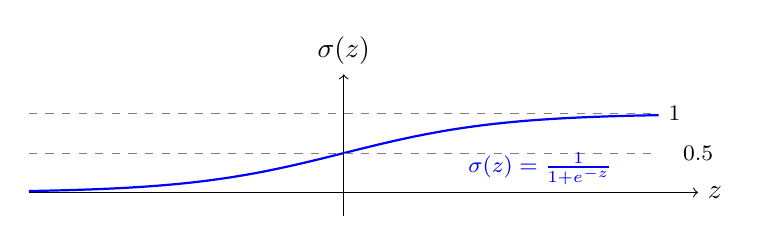
\begin{tikzpicture}
    \draw[->] (-4,0) -- (4.5,0) node[right] {$z$};
    \draw[->] (0,-0.3) -- (0,1.5) node[above] {$\sigma(z)$};
    \draw[blue, thick, domain=-4:4, smooth, samples=100] plot (\x, {1/(1+exp(-\x))});
    \draw[dashed, gray] (-4,1) -- (4,1);
    \draw[dashed, gray] (-4,0.5) -- (4,0.5);
    \node[font=\footnotesize] at (4.2, 1) {$1$};
    \node[font=\footnotesize] at (4.5, 0.5) {$0.5$};
    \node[font=\footnotesize, blue] at (2.5, 0.3) {$\sigma(z) = \frac{1}{1+e^{-z}}$};
\end{tikzpicture}
\end{center}

\begin{codeblock}[title=\textbf{Python}]
\begin{minted}{python}
from sklearn.linear_model import LogisticRegression
from sklearn.preprocessing import LabelEncoder

# Titanic: binary classification (survival)
titanic = sns.load_dataset('titanic').dropna(subset=['age', 'fare'])
X_ti = titanic[['age', 'fare', 'pclass']]
y_ti = titanic['survived']

X_train, X_test, y_train, y_test = train_test_split(
    X_ti, y_ti, test_size=0.3, random_state=42
)

logreg = LogisticRegression(max_iter=1000)
logreg.fit(X_train, y_train)
print(f"Accuracy (train): {logreg.score(X_train, y_train):.4f}")
print(f"Accuracy (test):  {logreg.score(X_test, y_test):.4f}")
\end{minted}
\end{codeblock}

\begin{codeoutput}
\begin{minted}{text}
Accuracy (train): 0.6962
Accuracy (test):  0.6878
\end{minted}
\end{codeoutput}

\section{Decision Trees}
\label{sec:arbres_decision}

\index{decision tree}\index{DecisionTreeClassifier}

\begin{definition}[Decision Tree]
A \textbf{decision tree} partitions the feature space through successive binary tests, forming a tree structure. Each leaf corresponds to a prediction.
\end{definition}

\begin{center}
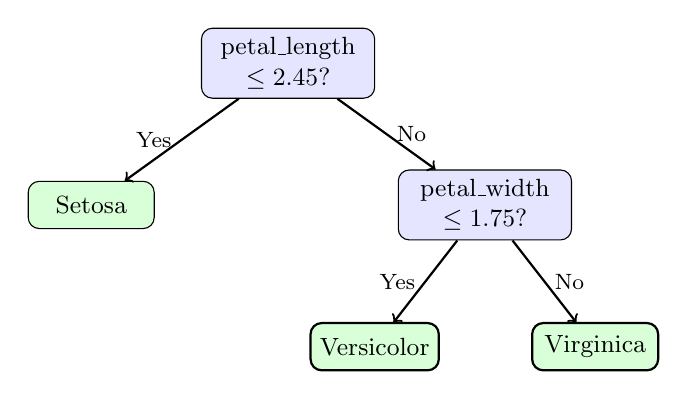
\begin{tikzpicture}[
    node/.style={rectangle, draw, rounded corners, fill=blue!10, minimum width=2.2cm, minimum height=0.7cm, align=center, font=\small},
    leaf/.style={rectangle, draw, rounded corners, fill=green!15, minimum width=1.6cm, minimum height=0.6cm, align=center, font=\small},
    edge from parent/.style={draw, ->, thick},
    level 1/.style={sibling distance=5cm, level distance=1.8cm},
    level 2/.style={sibling distance=2.8cm, level distance=1.8cm}
]
\node[align=center,node] {petal\_length\\$\leq 2.45$?}
    child {
        node[leaf] {Setosa}
        edge from parent node[left, font=\footnotesize] {Yes}
    }
    child {
        node[node] {petal\_width\\$\leq 1.75$?}
        child {
            node[leaf] {Versicolor}
            edge from parent node[left, font=\footnotesize] {Yes}
        }
        child {
            node[leaf] {Virginica}
            edge from parent node[right, font=\footnotesize] {No}
        }
        edge from parent node[right, font=\footnotesize] {No}
    };
\end{tikzpicture}
\end{center}

\begin{codeblock}[title=\textbf{Python}]
\begin{minted}{python}
from sklearn.tree import DecisionTreeClassifier
from sklearn.datasets import load_iris
from sklearn.model_selection import cross_val_score

iris = load_iris()
X, y = iris.data, iris.target

# Tree with limited maximum depth
tree = DecisionTreeClassifier(max_depth=3, random_state=42)
scores = cross_val_score(tree, X, y, cv=5)
print(f"Tree (max_depth=3): {scores.mean():.4f} (+/- {scores.std():.4f})")

# Tree without depth limit
tree_full = DecisionTreeClassifier(random_state=42)
scores_full = cross_val_score(tree_full, X, y, cv=5)
print(f"Tree (no limit):    {scores_full.mean():.4f} (+/- {scores_full.std():.4f})")
\end{minted}
\end{codeblock}

\begin{codeoutput}
\begin{minted}{text}
Tree (max_depth=3): 0.9667 (+/- 0.0211)
Tree (no limit):    0.9533 (+/- 0.0327)
\end{minted}
\end{codeoutput}

\begin{warning}
A tree without a depth limit (\py{max_depth=None}) risks \textbf{overfitting}. Limit the depth or the minimum number of samples per leaf (\py{min_samples_leaf}).
\end{warning}

\section{Random Forests}
\label{sec:forets_aleatoires}

\index{random forest}\index{RandomForestClassifier}\index{bagging}\index{ensemble}

\begin{definition}[Random Forest]
A \textbf{random forest} is an \textbf{ensemble} of $B$ decision trees trained on random subsamples of the data (\textit{bagging}). The final prediction is the \textbf{majority vote} (classification) or the \textbf{average} (regression).
\end{definition}

\begin{codeblock}[title=\textbf{Python}]
\begin{minted}{python}
from sklearn.ensemble import RandomForestClassifier

rf = RandomForestClassifier(n_estimators=100, max_depth=5, random_state=42)
scores_rf = cross_val_score(rf, X, y, cv=5)
print(f"Random forest: {scores_rf.mean():.4f} (+/- {scores_rf.std():.4f})")
\end{minted}
\end{codeblock}

\begin{codeoutput}
\begin{minted}{text}
Random forest: 0.9667 (+/- 0.0211)
\end{minted}
\end{codeoutput}

\section{K-Nearest Neighbors (KNN)}
\label{sec:knn_detail}

\index{KNN}\index{Euclidean distance}

\begin{definition}[KNN]
The \textbf{$k$-nearest neighbors} classifier assigns to a new observation the majority class among its $k$ nearest neighbors according to a distance metric (typically Euclidean):
\[
d(\mathbf{x}, \mathbf{x}') = \sqrt{\sum_{j=1}^{p}(x_j - x'_j)^2}
\]
\end{definition}

\begin{bestpractice}
KNN performance depends heavily on the \textbf{scale} of variables. Always normalize your data before using KNN:
\begin{minted}{python}
from sklearn.preprocessing import StandardScaler
scaler = StandardScaler()
X_scaled = scaler.fit_transform(X)
\end{minted}
\end{bestpractice}

\section{K-Means: Clustering}
\label{sec:kmeans}

\index{K-Means}\index{clustering}\index{elbow method}

\begin{definition}[K-Means]
\textbf{K-Means} is an \textbf{unsupervised} learning algorithm that partitions $n$ observations into $K$ groups (\textit{clusters}) by minimizing the inertia:
\[
\mathcal{J} = \sum_{k=1}^{K}\sum_{\mathbf{x}_i \in C_k} \| \mathbf{x}_i - \boldsymbol{\mu}_k \|^2
\]
where $\boldsymbol{\mu}_k$ is the centroid of cluster $C_k$.
\end{definition}

\begin{center}
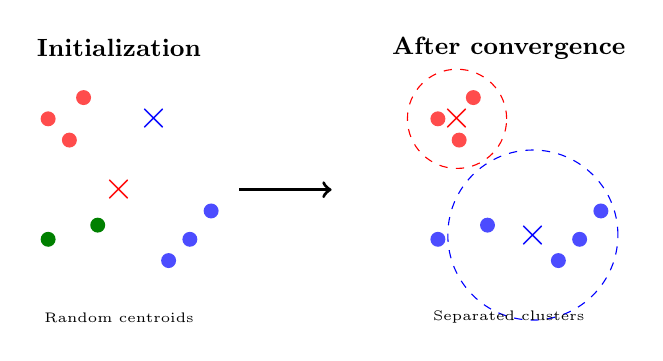
\begin{tikzpicture}[scale=0.9]
    % Iteration 1
    \begin{scope}[shift={(-4,0)}]
        \node[font=\bfseries\small] at (1.5, 3.5) {Initialization};
        \fill[red!70] (0.5, 2.5) circle (3pt);
        \fill[red!70] (1.0, 2.8) circle (3pt);
        \fill[red!70] (0.8, 2.2) circle (3pt);
        \fill[blue!70] (2.5, 0.8) circle (3pt);
        \fill[blue!70] (2.8, 1.2) circle (3pt);
        \fill[blue!70] (2.2, 0.5) circle (3pt);
        \fill[green!50!black] (1.2, 1.0) circle (3pt);
        \fill[green!50!black] (0.5, 0.8) circle (3pt);
        \node[red, font=\Large] at (1.5, 1.5) {$\times$};
        \node[blue, font=\Large] at (2.0, 2.5) {$\times$};
        \node[font=\tiny] at (1.5, -0.3) {Random centroids};
    \end{scope}
    % Arrow
    \draw[->, very thick] (-0.8, 1.5) -- (0.5, 1.5);
    % Iteration 2
    \begin{scope}[shift={(1.5,0)}]
        \node[font=\bfseries\small] at (1.5, 3.5) {After convergence};
        \fill[red!70] (0.5, 2.5) circle (3pt);
        \fill[red!70] (1.0, 2.8) circle (3pt);
        \fill[red!70] (0.8, 2.2) circle (3pt);
        \fill[blue!70] (2.5, 0.8) circle (3pt);
        \fill[blue!70] (2.8, 1.2) circle (3pt);
        \fill[blue!70] (2.2, 0.5) circle (3pt);
        \fill[blue!70] (1.2, 1.0) circle (3pt);
        \fill[blue!70] (0.5, 0.8) circle (3pt);
        \node[red, font=\Large] at (0.77, 2.5) {$\times$};
        \node[blue, font=\Large] at (1.84, 0.86) {$\times$};
        \draw[red, dashed] (0.77, 2.5) circle (0.7cm);
        \draw[blue, dashed] (1.84, 0.86) circle (1.2cm);
        \node[font=\tiny] at (1.5, -0.3) {Separated clusters};
    \end{scope}
\end{tikzpicture}
\end{center}

\begin{codeblock}[title=\textbf{Python}]
\begin{minted}{python}
from sklearn.cluster import KMeans
from sklearn.datasets import load_iris
import numpy as np

iris = load_iris()
X = iris.data

# Elbow method
inertias = []
K_range = range(1, 11)
for k in K_range:
    km = KMeans(n_clusters=k, n_init=10, random_state=42)
    km.fit(X)
    inertias.append(km.inertia_)

print("K  | Inertia")
print("-" * 20)
for k, inertia in zip(K_range, inertias):
    print(f"{k:2d} | {inertia:.1f}")
\end{minted}
\end{codeblock}

\begin{codeoutput}
\begin{minted}{text}
K  | Inertia
--------------------
 1 | 681.4
 2 | 152.3
 3 | 78.9
 4 | 57.3
 5 | 46.5
 6 | 39.0
 7 | 34.2
 8 | 29.9
 9 | 27.8
10 | 25.4
\end{minted}
\end{codeoutput}

\begin{intuition}
The \textbf{elbow method}\index{elbow method} consists of finding the point where the inertia stops decreasing significantly. Here, $K=3$ corresponds to the ``elbow'', consistent with the 3 Iris species.
\end{intuition}

\section{Model Comparison Table}

\begin{center}
\begin{tabular}{llccc}
\toprule
\textbf{Model} & \textbf{Type} & \textbf{Interpretable} & \textbf{Normalization} & \textbf{Key hyperparameters} \\
\midrule
Linear reg. & Regression & Yes & No & --- \\
Logistic reg. & Classification & Yes & Yes & \py{C} \\
Decision tree & Both & Yes & No & \py{max_depth} \\
Random forest & Both & No & No & \py{n_estimators}, \py{max_depth} \\
KNN & Both & No & Yes & \py{n_neighbors} \\
K-Means & Clustering & Medium & Yes & \py{n_clusters} \\
\bottomrule
\end{tabular}
\end{center}

\section{Exercises}

\begin{exercise}[$\star$]
Load the \texttt{tips} dataset from seaborn. Train a linear regression to predict the tip (\py{tip}) from \py{total_bill} only. Display the coefficient, intercept, and $R^2$.
\end{exercise}

\begin{exercise}[$\star$]
On the Iris dataset, compare the accuracy (5-fold cross-validation) of a decision tree (\py{max_depth=3}), a random forest (100 trees), and KNN ($k=5$).
\end{exercise}

\begin{exercise}[$\star\star$]
Load the \texttt{titanic} dataset from seaborn. Prepare the data (remove rows with missing values in \py{age}, \py{fare}; use \py{pclass}, \py{age}, \py{fare}, \py{sex} encoded). Compare logistic regression and a random forest for predicting \py{survived}.
\end{exercise}

\begin{exercise}[$\star\star$]
Apply K-Means with $K=3$ on the Iris data (without labels). Compare the obtained clusters with the true species using a cross-tabulation (\py{pd.crosstab}).
\end{exercise}

\begin{exercise}[$\star\star\star$]
Load the \py{fetch_california_housing()} dataset from scikit-learn. Train a linear regression and a random forest. Compare the $R^2$ and RMSE on the test set. Plot predictions vs.\ actual values for both models.
\end{exercise}

\begin{exercise}[$\star\star\star$]
Implement the KNN algorithm ``from scratch'' (without scikit-learn) using NumPy. Test it on Iris and compare your results with \py{KNeighborsClassifier}.
\end{exercise}

\begin{keyformulas}
\textbf{Summary of Chapter~\ref{ch:modeles}}
\begin{itemize}
    \item \textbf{Linear regression}: $y = \mathbf{X}\boldsymbol{\beta} + \varepsilon$, OLS: $\hat{\boldsymbol{\beta}} = (\mathbf{X}^\top\mathbf{X})^{-1}\mathbf{X}^\top\mathbf{y}$.
    \item \textbf{Logistic regression}: $P(y{=}1|\mathbf{x}) = \sigma(\mathbf{x}^\top\boldsymbol{\beta})$, binary classification.
    \item \textbf{Decision tree}: successive partitions, control \py{max_depth}.
    \item \textbf{Random forest}: ensemble of trees via \textit{bagging}, more robust.
    \item \textbf{KNN}: vote of $k$ nearest neighbors, requires normalization.
    \item \textbf{K-Means}: unsupervised clustering, minimizes inertia $\mathcal{J}$.
    \item \textbf{Elbow method}: choose $K$ at the inflection point of the inertia.
\end{itemize}
\end{keyformulas}
